\documentclass[11pt]{article}

\usepackage[margin=1in]{geometry}
\usepackage[numbers,sort&compress]{natbib}
\usepackage{graphicx}
\usepackage{float}
\usepackage{booktabs}
\usepackage{amsmath}
\usepackage{microtype}
\usepackage[hidelinks]{hyperref}
\usepackage{xcolor}

\newcommand{\claimed}{\textit{claimed}}
\newcommand{\audited}{\textit{audited}}

\title{When Self-Reported Fitness Becomes the Target:\\
Independent Audits in LLM-Driven Recipe Evolution}
\author{Qindong Gan\\
Waseda University\\
\texttt{ganqindong@fuji.waseda.jp}}
\date{September 2026}

\begin{document}
\maketitle

\begin{abstract}
LLM-driven program evolution requires a score for deciding which generated programs reproduce.
That score need not be comparable when each program controls part of its own measurement. We
study this failure mode in a small reinforcement-learning system where an LLM rewrites training
recipes for a fixed LunarLander policy trainer. Every trained policy receives both a training
score and a harness-owned audit: 32 fresh-seed episodes scored only by raw environment reward,
with no recipe-code execution. We compare audit-based against training-score-based selection in
two reward-source protocols, using three independent 15-candidate outer loops per cell. With
candidate-shaped training reward, claimed scores saturated at $10^9$ and the final audited return
averaged $4.0$ under audit selection versus $-762.1$ under claimed selection; claimed-selection
regret averaged $710.4$. A fixed-raw control removed candidate reward shaping and score
saturation. The gap narrowed but did not disappear: final audited return averaged $-19.4$ versus
$-137.1$, and claimed-selection regret averaged $110.7$, with a selection error in all three
runs. The comparison identifies candidate-defined reward scale as a major amplifier, not the only
source, of self-report misranking. This is a reproducible mechanism-and-ablation case study, not
a population estimate: each cell has only three runs, all in one environment with one model
configuration, and the two protocols were run at different times.
\end{abstract}

\section{Introduction}

Large language models increasingly propose programs inside search loops: mathematical programs,
algorithms, prompts, reward functions, and components of automated research
systems~\citep{romeraparedes2024funsearch,novikov2025alphaevolve,real2020automlzero,
yang2024opro,ma2024eureka,lu2024aiscientist}. These systems depend on a selection score. With an
exact verifier or a fixed benchmark harness, candidates share a trusted objective. With training
programs, however, a tempting shortcut is to archive the best score reported during each
candidate's own run.

Self-reporting is dangerous when candidates can change reward shaping, evaluation horizon, sample
count, or seeds. The score then mixes policy quality with a candidate-specific unit of
measurement. Selection pressure can favor the report rather than the underlying policy---a direct
Goodhart-style failure~\citep{manheim2018categorizing} related to specification gaming and reward
hacking~\citep{krakovna2020specification,lehman2020surprising,skalse2022defining,
pan2022effects,amodei2016concrete}. Unlike an agent that edits evaluator code, the candidates in
our system obey their declared interface. The problem is more basic: the interface permits each
candidate to define a different proxy scale.

We test the smallest structural remedy: keep candidate-controlled training, but add a separate
evaluation path that receives only the trained policy parameters, uses fresh seeds, and scores raw
environment reward. We call this path an \emph{audit}. The experiment changes only which score
drives parent selection and LLM feedback. Audits are still recorded in both selection conditions.
We then repeat the comparison with candidate reward shaping disabled, so that the training score
is raw environment reward while candidates can still choose optimizer and evaluation schedules.

Our contributions are:
\begin{enumerate}
  \item a compact, open implementation of audit-gated LLM recipe evolution with immutable run
  configuration, prompt hashing, resumable outer-loop randomness, and per-episode audit records;
  \item twelve LunarLander outer-loop runs in a $2\times2$ design---audit versus training-score
  selection, crossed with candidate-shaped versus fixed-raw training reward---with three
  independent runs and 15 candidates per cell;
  \item a tie-aware analysis showing that claim-based selection becomes scale-saturated under
  candidate shaping, while avoiding the unsupported assertion that every highly shaped candidate
  is a poor policy; and
  \item a fixed-raw ablation showing substantially smaller but persistent selection errors after
  candidate reward content and scale are removed, plus reproducibility bundles containing all
  180 candidate recipes, trained parameter vectors, audit records, and provenance metadata.
\end{enumerate}

The study is intentionally narrow. Three runs per cell support a reproducible case study and
effect-size description, not formal inference or broad claims about LLMs, reinforcement learning,
or program evolution.

\section{System}
\label{sec:system}

\begin{figure}[H]
\centering
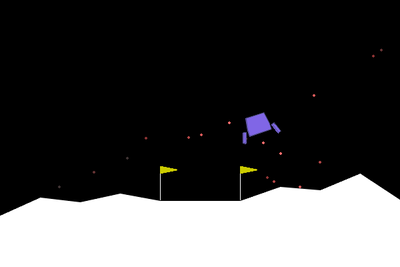
\includegraphics[width=0.45\textwidth]{../assets/lunarlander_audit_replay.png}
\caption{Illustrative LunarLander-v3 frame from one archived audit episode (audited-selection
outer seed 101, candidate 9, episode seed 995252232). The episode's raw return was 190.06.
This image is an environment preview, not an additional experiment or the 32-episode mean.}
\label{fig:lunar-preview}
\end{figure}

\paragraph{Recipe contract.}
A candidate is a Python module defining three components: (i) separable CMA-ES settings
($\sigma_0\in[0.01,2]$, population size 4--64); (ii) a generation-dependent schedule specifying
1--16 evaluation episodes and a 50--1000 step training horizon; and (iii) a deterministic
per-transition shaped-reward function. Shaped reward must be finite and have magnitude at most
$10^6$ per transition. The candidate cannot change the policy architecture, trainer, total
episode budget, audit, or archive.

Generated code passes AST hygiene checks, import/loading checks, and dynamic contract probes.
These checks are not a security sandbox; experiments should run on trusted infrastructure. If a
proposal fails, the next rejection-sampling prompt includes the validator's reason. The complete
static prompt is hashed into the immutable run configuration.

\paragraph{Fixed inner trainer.}
The policy is a tanh multilayer perceptron with layers $(8,32,32,4)$, totaling 1,476 parameters.
It is trained with separable CMA-ES~\citep{hansen2001cmaes,ros2008sepcma}, following the broader
use of evolution strategies for policy search~\citep{salimans2017evolution}. A candidate receives
at most 2,000 training episodes and 600 wall-clock seconds. Population members are evaluated on a
small, fixed training seed pool under that recipe's shaped reward and schedule.

\paragraph{Two reward sources.}
The primary candidate-shaped protocol executes each recipe's shaped-reward function during
training. The fixed-raw control instead substitutes raw environment reward inside the trainer and
never calls candidate shaping. Candidates in both protocols can still choose CMA-ES settings,
evaluation episodes, and horizon schedules. The control therefore removes candidate-defined
reward content and scale together; it does not hold every other source of training noise fixed.

\paragraph{Two selection scores.}
The \claimed{} score is the highest training fitness observed in the candidate's run. The
submitted parameters are also those judged best by that signal. The \audited{} score is the
mean raw environment return from 32 new seeds drawn from OS entropy, using a fixed 1000-step
horizon. Audit code receives the policy parameters but does not import or call the recipe. For a
candidate $i$, we record the honesty gap
\[
g_i = c_i-a_i,
\]
where $c_i$ is its reported best training score and $a_i$ its audit. Under fixed raw reward,
$c_i$ is the raw training return of the submitted policy, but it remains the best noisy estimate
observed on reused training seeds. Under candidate shaping, scores need not share units, so
$g_i$ is a diagnostic rather than a calibrated estimate of lying or intent.

\paragraph{Outer loop.}
Each run begins with a hand-written raw-reward seed recipe. The outer loop selects a parent (80\%
uniformly from the current top five, 20\% from the whole completed archive), gives the LLM the
parent source and its selection score, validates the proposed child, trains it, audits it, and
appends a record. In \textbf{audited selection}, parent ranking and feedback use $a_i$. In
\textbf{claimed selection}, both use $c_i$; audits remain hidden from selection and are recorded
only for analysis. After 15 completed candidates, the system returns the archive maximum under
the selected signal. Python's stable ordering resolves exact score ties by earlier archive order.

\section{Experimental protocol}
\label{sec:protocol}

Table~\ref{tab:protocol} summarizes the two experimental phases. LunarLander-v3 uses Gymnasium's
discrete four-action task and raw environment return~\citep{towers2024gymnasium}. Protocol v3
uses candidate-shaped training rewards; protocol v4 is the fixed-raw control. Within each phase,
we used outer-loop RNG seeds 101, 202, and 303 in both selection modes. The same seed labels align
some harness random streams, but neither the within-phase comparison nor the cross-phase ablation
is strictly paired: model sampling is stochastic, audit seeds come independently from OS entropy,
and the phases were run on different dates with different static prompts.

\begin{table}[t]
\centering
\small
\begin{tabular}{lll}
\toprule
Item & Candidate-shaped (v3) & Fixed-raw (v4) \\
\midrule
Environment & \multicolumn{2}{c}{LunarLander-v3, discrete actions} \\
Selection modes & \multicolumn{2}{c}{audited, claimed} \\
Independent runs & \multicolumn{2}{c}{3 per cell (seeds 101, 202, 303)} \\
Candidates & \multicolumn{2}{c}{15 completed candidates per run} \\
Training budget & \multicolumn{2}{c}{2,000 episodes, 600 s per candidate} \\
Audit & \multicolumn{2}{c}{32 fresh seeds, raw reward, 1,000-step horizon} \\
Training reward & candidate shaped & raw environment reward \\
Mutation requests & 84 & 84 \\
Prompt fingerprint & \texttt{be9c5020...a00e8a} & \texttt{f420fda4...107df} \\
\bottomrule
\end{tabular}
\caption{Experimental design. Both phases used Codex CLI 0.146.0, \texttt{gpt-5.6-sol}, and low
reasoning. A run, not a candidate or audit episode, is the unit of replication.}
\label{tab:protocol}
\end{table}

For each run we report: (i) the raw-reward audit of the candidate actually selected by that
mode; (ii) the best audit observed anywhere in the same archive (an oracle available only after
recording audits); and (iii) selection regret, the oracle audit minus the selected candidate's
audit. Audited selection has zero within-archive regret by construction, so its zero is not an
empirical discovery. The informative questions are the audited quality of each mode's final pick
and whether claimed scores preserve enough ordering information to select among their own
archive.

We provide no candidate-level $p$-values: candidates share ancestry, and the 32 audit episodes
measure one submitted policy rather than 32 independent evolution runs. With only three outer
runs per cell, all between-mode and cross-protocol summaries are descriptive.

\section{Results}
\label{sec:results}

\subsection{Final selected policies}

The audit-selected final policies scored $33.0$, $-48.7$, and $27.6$ on raw environment reward
(mean $4.0$). The claim-selected final policies scored $-1102.3$, $-422.7$, and $-761.4$
(mean $-762.1$). The seed-aligned audited-minus-claimed differences were $1135.3$, $374.0$, and
$789.0$ points (Figure~\ref{fig:selected}). These are large realized differences, but three
stochastic runs do not establish their population frequency or expected magnitude.

\begin{figure}[t]
\centering
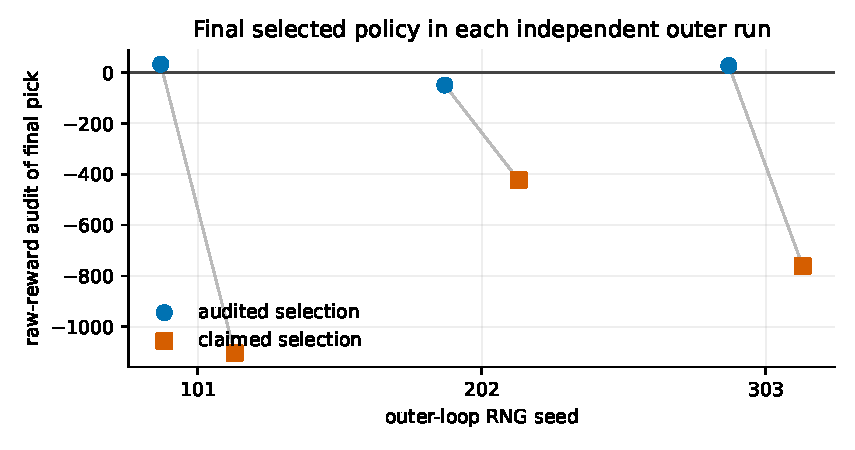
\includegraphics[width=0.82\textwidth]{figs/v3_selected_outcomes.pdf}
\caption{Raw-reward audit of the final candidate returned by each selection rule. Lines align
the same outer-loop RNG seed, but model samples and audit seeds are not paired.}
\label{fig:selected}
\end{figure}

\begin{table}[t]
\centering
\small
\begin{tabular}{rrrrr}
\toprule
Seed & audited-mode pick & claimed-mode pick & claimed-run oracle & actual regret \\
\midrule
101 & $33.0$ & $-1102.3$ & $-111.5$ & $990.8$ \\
202 & $-48.7$ & $-422.7$ & $-85.4$ & $337.3$ \\
303 & $27.6$ & $-761.4$ & $41.6$ & $802.9$ \\
\midrule
Mean & $4.0$ & $-762.1$ & $-51.8$ & $710.4$ \\
\bottomrule
\end{tabular}
\caption{Run-level outcomes in raw LunarLander reward. ``Oracle'' is the best audited candidate
already present in the claimed-selection archive; it is post-hoc and was unavailable to that
selection rule.}
\label{tab:outcomes}
\end{table}

\subsection{Claim saturation destroys ranking information}

In all three claimed-selection runs, generated recipes reached a claimed score of exactly
$10^9$. This value follows from the contract rather than a validator escape: a recipe may emit a
shaped reward of $10^6$ at each of 1000 steps. The resulting number is a valid shaped-training
return but has no raw-reward interpretation. Candidate-level scores separate sharply by mode in
Figure~\ref{fig:mechanism}a: audited selection still produces optimistic claims, whereas claimed
selection drives many candidates to the allowed scale ceiling.

The highest claimed score was tied by 5, 2, and 3 candidates in seeds 101, 202, and 303. The
implemented stable tie-break selected the earliest, producing regrets of $990.8$, $337.3$, and
$802.9$ (Table~\ref{tab:outcomes}). To avoid attributing the full result to that arbitrary
tie-break, we also compute a favorable bound: retrospectively choose the best audited policy among
all candidates tied at the maximum claim. The remaining regrets are $1.2$, $337.3$, and $273.8$
(mean $204.1$). Thus, even an audit-informed tie-break among top claims would fail to recover the
archive oracle in every run (Figure~\ref{fig:mechanism}b). Once reports saturate, the claimed metric
cannot distinguish policies that differ by hundreds of raw-reward points.

\begin{figure}[t]
\centering
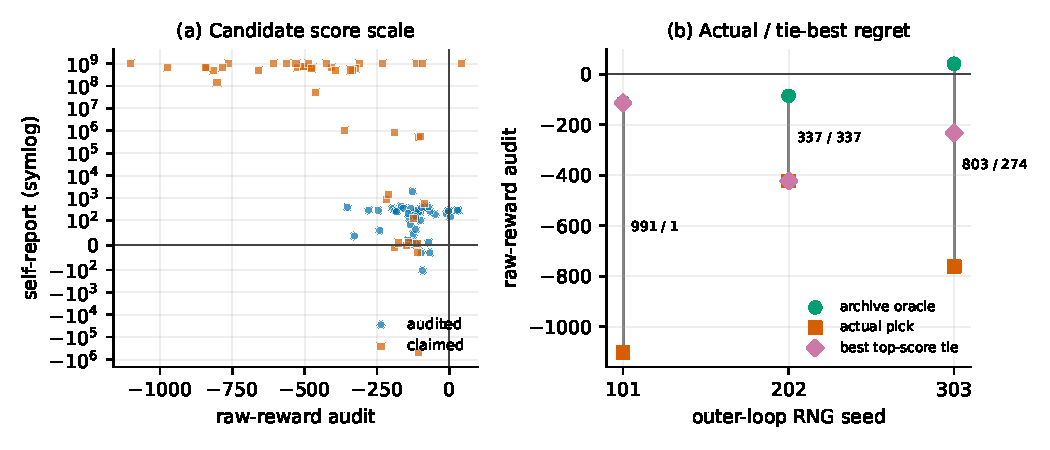
\includegraphics[width=\textwidth]{figs/v3_mechanism.pdf}
\caption{Mechanism evidence. (a) All 90 candidates; the self-report axis uses a symmetric log
scale. Points are dependent within outer runs. (b) Within each claimed-selection archive: actual
stable-tie pick, best audited candidate among maximum-claim ties, and overall audit oracle. Labels
show actual / tie-favorable regret.}
\label{fig:mechanism}
\end{figure}

This is a comparability failure, not proof that large shaping always produces a poor policy. One
candidate in seed 303 claimed $9.999\times 10^8$ and audited at $41.6$, the best raw-reward policy
in that archive. Other nearly identical claims audited hundreds of points lower. The issue is
precisely that the claimed score cannot tell them apart.

\subsection{Fixed-raw reward-source ablation}

The fixed-raw phase asks whether candidate-defined reward content and scale are necessary for the
selection failure. They are not. Under audit selection, final-policy audits were $-6.7$, $-69.3$,
and $17.9$ (mean $-19.4$). Under claimed selection they were $-166.9$, $-140.1$, and $-104.2$
(mean $-137.1$). In all three claimed-selection runs, another candidate in the same archive had a
higher audit. Selection regrets were $172.3$, $86.0$, and $73.9$ (mean $110.7$).

\begin{table}[t]
\centering
\small
\begin{tabular}{rrrrr}
\toprule
Seed & audited-mode pick & claimed-mode pick & claimed-run oracle & regret \\
\midrule
101 & $-6.7$ & $-166.9$ & $5.4$ & $172.3$ \\
202 & $-69.3$ & $-140.1$ & $-54.1$ & $86.0$ \\
303 & $17.9$ & $-104.2$ & $-30.3$ & $73.9$ \\
\midrule
Mean & $-19.4$ & $-137.1$ & $-26.3$ & $110.7$ \\
\bottomrule
\end{tabular}
\caption{Fixed-raw control outcomes. ``Claimed'' now means the best raw training return observed
on the training seed pool, not candidate-shaped reward. The oracle remains post-hoc.}
\label{tab:fixedraw}
\end{table}

\begin{figure}[t]
\centering
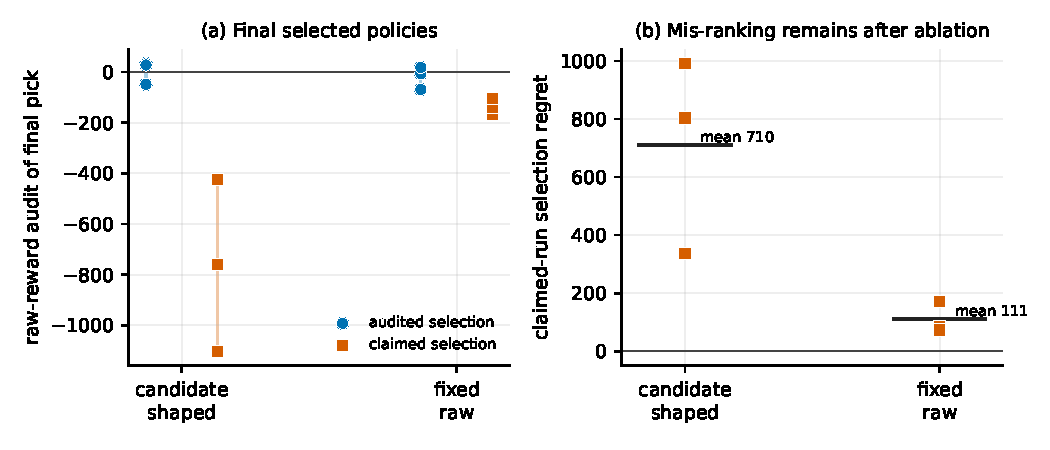
\includegraphics[width=\textwidth]{figs/v3_v4_ablation.pdf}
\caption{Reward-source ablation. Points are independent outer runs ($n=3$ per cell); bars show
means. Candidate shaping creates score saturation and much larger realized regret. Fixed raw
reward removes saturation but not all misranking between noisy training scores and fresh audits.}
\label{fig:ablation}
\end{figure}

Figure~\ref{fig:ablation} supports a layered account. Candidate-defined reward scale is a major
amplifier: removing it reduced mean claimed-selection regret from $710.4$ to $110.7$ and reduced
the mean final-policy gap between selection modes from $766.1$ to $117.7$. It is not the sole
source: the fixed-raw claimed score is still the maximum observed training estimate, often based
on one episode at the selected best generation, on reused training seeds and candidate-chosen
schedules. These features are plausible explanations, not separately randomized causal findings.
Because the v3 and v4 phases used different prompts and were run at different times, the numerical
reduction itself should not be read as a clean paired estimate of reward shaping's causal effect.

\subsection{What the experiment does and does not show}

The experiment directly shows that the permitted candidate-controlled metric can saturate and
that selecting on it can return a much worse audited policy than one already trained in the same
run. The fixed-raw phase further shows that raw training scores can still misrank policies relative
to a fresh-seed audit. A harness-owned audit preserves a common unit and separates selection from
the training measurement. The study does \emph{not} isolate every remaining cause, prove that
audit selection improves search in expectation, or show that selected recipes reproduce their
policy quality when retrained.

The repository also contains historical MinAtar Breakout~\citep{young2019minatar} pilot archives
using a gymnax backend~\citep{lange2022gymnax}. Those pilots have only one outer run per mode and
predate protocol-v3 metadata. They demonstrate that the harness supports a second environment and
execution backend, but we do not pool them with the primary experiment or claim cross-environment
replication.

\section{Reproducibility and provenance}

Every replicated run stores an immutable configuration, Python and package versions, mutation
provider, CLI version, model identifier, reasoning setting, full static-prompt hash, outer-loop
RNG checkpoint, complete training history, audit seeds, per-episode raw returns, candidate source,
and trained parameters. Rerunning with a changed configuration is rejected rather than silently
mixing protocols. The 12 included runs contain exactly 180 completed candidates and no failed
records.

Across both phases, the mutation operator made 168 requests totaling 2,988,801 recorded input
tokens and 77,263 output tokens; all passed validation on the first attempt. Authentication used a
local ChatGPT login, but no secret or credential is stored in the archives. Separate public
replication bundles are sanitized for machine-local paths, licensed under Apache-2.0, checked for
restricted keywords and secret-like values, and accompanied by per-file hashes plus deterministic
archive checksums. The analysis scripts reconstruct Tables~\ref{tab:outcomes} and
\ref{tab:fixedraw} directly from the bundles without executing generated recipes.

\section{Limitations}

\textbf{Three runs per cell.} The consistency and magnitude observed here motivate further
work but do not justify asymptotic, statistical-significance, or generality claims.
\textbf{One replicated environment.} Breakout remains a historical pilot; the primary evidence is
LunarLander only.
\textbf{Joint rather than surgical ablation.} Fixed raw reward removes both shaping content and
scale. It does not distinguish scale normalization from removing shaping altogether.
\textbf{Not strictly paired.} Reusing outer RNG seed labels does not fix stochastic model outputs
or fresh audit seeds. The two phases also used different prompts and dates, so seed-aligned and
cross-protocol differences are descriptive rather than randomized paired estimates.
\textbf{One model configuration.} The recorded identifier is a service model name, not an
immutable server-weight snapshot; CLI version, date, prompt hash, and generated sources provide
the available provenance.
\textbf{Audits certify policies, not recipes.} A fresh-seed audit measures one trained parameter
vector. Stable recipe quality would require independent retraining of finalists.
\textbf{Generated code.} Static checks are hygiene, not adversarial containment. The system should
not execute candidates near secrets or untrusted resources.

\section{Related work}

Program-evolution systems with exact or harness-owned evaluators include FunSearch and
AlphaEvolve~\citep{romeraparedes2024funsearch,novikov2025alphaevolve}; AutoML-Zero similarly
evaluates evolved algorithms inside a controlled pipeline~\citep{real2020automlzero}. Eureka
uses LLM-generated reward functions but judges them by policies trained and evaluated under a
fixed outer procedure~\citep{ma2024eureka}, structurally closer to our audited condition. Our
claimed condition instead exposes what happens when a candidate-defined training metric becomes
the selection metric itself.

The observed failure belongs to the broader family of reward hacking, specification gaming, and
Goodhart effects~\citep{krakovna2020specification,skalse2022defining,pan2022effects,
lehman2020surprising,manheim2018categorizing}. Automated-science systems have exhibited adjacent
failures such as modifying evaluation code~\citep{lu2024aiscientist}. Here candidates need not
violate the interface: optimizing an allowed measurement scale is enough. The audit gate is the
minimal architectural separation between candidate-controlled optimization and a comparable
selection signal.

\section{Conclusion}

When LLM-generated training recipes control reward shaping, their self-reported fitness values
need not share a meaningful scale. Candidate-shaped runs drove reports to the contract ceiling and
selected policies whose raw-reward audits were far below alternatives already in the archives.
Fixed raw reward removed saturation and sharply reduced the observed damage, but training-score
selection still misranked the archive in all three runs. The evidence therefore supports a layered
failure: candidate-defined scale can dominate selection, while noisy best-of-training estimates
can remain misaligned with fresh-seed policy quality. A separate audit using fresh seeds, raw
rewards, and no recipe-code path restores a common selection measurement. Broader claims require
more environments, models, outer runs, a randomized reward-scale control, and finalist retrains.

\paragraph{Artifacts.}
Code, analysis, and release instructions are available at
the \href{https://github.com/Frankiegan912/shinsa-evolve}{project repository}. Separate protocol-v3
and protocol-v4 data bundles contain the complete replicated evidence and deterministic SHA-256
checksums.

\small
\bibliographystyle{plainnat}
\bibliography{references}

\end{document}
